%%
%% Edward T. Norris
%% Discrete Ordinates Computed Tomography Organ Dose Simulator (DOCTORS)
%% 
%% === Methods ===
%%

This chapter summarizes the solution methodology employed by DOCTORS. The techniques used to compute the collided and uncollided fluxes are described in separate sections. After the flux solution methodology is explained, the methods used for source generation and flux-to-dose conversion are covered.

\section{Discrete Ordinate Methods}

The discrete ordinate solver computes the flux distribution inside the CT mesh given a source, physical geometry information, and other associated solver parameters such as quadrature and energy discretization. Discrete ordinates is a deterministic solution to the linear Boltzmann equation.

\subsection{The Boltzmann Equation}

The linear Boltzmann equation (LBE) is generally true of any particle given that outside forces (electromagnetic or gravitational) are either not present or negligible and particle-particle collisions are insignificant. Therefore, the LBE is generally not valid for charged particles or systems whose particle density is on the order of the medium they are traveling through. In such systems, particle-particle interactions may not be negligible.  

In general, the LBE is valid for multiplying media (such as neutrons passing through fuel in a reactor), but the variant considered in this work omits such terms since only photons in medical systems are of concern. Solutions to the LBE can also be used to solve criticality eigenvalue problems or to produce adjoint parameters for other codes. Such solutions are not considered in this work.

The steady state form of the LBE can be readily derived from simple intuition. In the steady state, particle production and removal must be equal. In any volume, three production mechanisms are present. Particles can (1) stream into the volume across a bounding surface, (2) inscatter from another energy-direction component of phase space, or (3) be produced directly by the external source. Three removal terms are also present, particles can (1) stream out of the volume of interest by crossing a bounding surface, (2) be absorbed and vanish entirely, or (3) outscatter to a energy-direction component of phase space other than the one of interest.

The downscatter and absorption removal terms are typically grouped together using
\begin{equation}
\Sigma_t = \Sigma_a + \Sigma_s
\end{equation}
where $\Sigma_t$, $\Sigma_a$, and $\Sigma_s$ are the macroscopic total, absorption, and scatter cross sections respectively. The removal of particles from interactions (scatter and absorption) per volume is then
\begin{equation}
\Sigma_t(\boldsymbol{r}, E) \psi(\boldsymbol{r}, E, \hat{\Omega})
\end{equation}
where $\psi$ is the angular flux. The production and removal streaming operators are combined as 
\begin{equation}
\hat{\Omega} \cdot \nabla \psi(\boldsymbol{r}, E, \hat{\Omega})
\end{equation}
and included as a removal term since the normal is defined pointing outward from the volume. The normal sign convention results in particles streaming out being positive and those streaming in becoming negative. 

The inscatter to a particular energy and direction is computed by integrating over all other energies and directions
\begin{equation}
\int_{4\pi}^{} \int_{0}^{\infty} \Sigma_s(\boldsymbol{r}, E' \rightarrow E, \hat{\Omega}' \rightarrow \hat{\Omega}) \psi(\boldsymbol{r}, E', \hat{\Omega}') dE' d\hat{\Omega}'.
\end{equation}
An external source $S$ produces particles per volume. Combining the removal terms on the left and the production terms on the right yields
\begin{equation} \label{eq:boltz}
\begin{split}
	&\left[ \hat{\Omega} \cdot \nabla + \Sigma_t(\boldsymbol{r}, E) \right]
	\psi(\boldsymbol{r}, E, \hat{\Omega}) = \\
	&\int_{4 \pi} \int_0^\infty \Sigma_s(\boldsymbol{r}, E' \rightarrow E, \hat{\Omega}' \rightarrow \hat{\Omega}) \psi(\boldsymbol{r}, E', \hat{\Omega}') dE' d\hat{\Omega}' + S(\boldsymbol{r}, E, \hat{\Omega})
\end{split}
\end{equation}
which is the LBE. The following sections show how Eq.~\ref{eq:boltz} is discretized and solved computationally.

\subsection{Angular Discretization}
The coordinate system used in DOCTORS is shown in Fig.~\ref{fig:coord_sys}. A discrete set of $N_a$ angles ($\Omega_{a}, \quad a = 0 \ldots N_a-1$) is selected to represent continuous directional space. Particles are transported only along these discrete directions from each voxel to adjacent voxels.

\begin{figure}[tb]
  \begin{center}
   \includegraphics[width=3.75in]{figs/coord_sys}
  \end{center}
  \caption{The coordinate system used in DOCTORS. Given an arbitrary direction, $\Omega$, $\mu$, $\eta$, and $\xi$ are its direction cosines with respect to the $x$, $y$, and $z$ axes respectively. $\varphi$ is the azimuthal angle (with respect to $x$ and the d $\theta$ is the polar angle (with respect to $z$).}
\label{fig:coord_sys}
\end{figure}

The rotation symmetrical quadrature is implemented in DOCTORS. From amongst many different quadrature sets, the rotation symmetrical quadratures were selected because they are easy to implement, rotationally symmetric, and the most commonly used in production discrete ordinate solvers [CITE] which enables simple, direct comparison to other solvers. Arbitrary quadratures are permissible in a plain text file supplied by the user enabling other quadratures.

THEORY AND MATH OF ANGLE/WEIGHT GENERATION?

To include a user defined quadrature, the plain text file should be formatted such that it contains four columns similar to Table~\ref{tab:quad_format} (without any headings). No checks are performed to ensure that octants are covered, this allows simple testing quadratures that utilize only a single direction to be used. Values for $\mu$, $\eta$, and $\xi$ do not necessarily need to add to unity as they will be automatically normalized by DOCTORS. Likewise, the weights will be normalized such that their summation is unity. However, user defined directions \textit{should not} be parallel to any major axis. Doing so may result in undefined behavior. Also, after normalization, no two rows should have identical values for $\mu$, $\eta$, and $\xi$ such as the last two rows of Table~\ref{tab:quad_interp}, nor may any weights be negative. The data in Table~\ref{tab:quad_format} would be read in and renormalized by DOCTORS. The normalized data would be identical to the data in Table~\ref{tab:quad_interp}.

Values are read in as a 32 bit IEEE-754 floating point number [CITE] which ensures seven significant digits. Significant digits beyond this will be truncated. Note that Table~\ref{tab:quad_interp} rounds four digits after the decimal.

\begin{table}[ht]
\caption{User Defined Quadrature Input}
\centering 
\begin{tabular}{c c c c}
\hline \hline   
$\mu$    & $\eta$ & $\xi$ & Weight\\ [0.5ex] 
\hline
1        & 0      & 0      & 1 \\
0.999    & 0.001  & 0.001  & 1 \\
1.0      & 1.0    & 1.0    & 1.3 \\
0.02198  & 0.2987 & .34520 & .02226 \\
.001     & .001   & .999   & 0.999 \\
-1       & 1      & -1     & .2 \\
-1.2     & 1.2    & -1.2   & 0.1 \\
-1        & 1     & -1     & .2 \\ [1ex]
\hline
\end{tabular}
\label{tab:quad_format}
\end{table}

\begin{table}[ht]
\caption{User Defined Quadrature Interpretation}
\centering 
\begin{tabular}{c c c c}
\hline \hline   
$\mu$    & $\eta$ & $\xi$ & Weight\\ [0.5ex] 
\hline
 1.0000  &  0.0000  &  0.0000  & 0.2074 \\
 1.0000  &  0.0010  &  0.0010  & 0.2074 \\
 0.5774  &  0.5774  &  0.5774  & 0.2696 \\
 0.0481  &  0.6536  &  0.7553  & 0.0207 \\
 0.5000  & -0.5000  &  0.7071  & 0.0046 \\
 0.5774  & -0.5774  & -0.5774  & 0.2072 \\
-0.5774  &  0.5774  & -0.5774  & 0.0415 \\
-0.5774  &  0.5774  & -0.5774  & 0.0415 \\ [1ex]
\hline
\end{tabular}
\label{tab:quad_interp}
\end{table}

A given direction, $\hat{\Omega}$, is determined by its three cosine components: 
\begin{equation} \label{eq:omega_cos}
\hat{\Omega} = \mu \hat{i} + \eta \hat{j} + \xi \hat{k}
\end{equation}
where $\hat{i}$, $\hat{j}$, and $\hat{k}$ are the unit directions in the $x$, $y$, and $z$ directions respectively. Therefore, any discrete direction $\hat{\Omega}_a$ can be expressed as $<\mu, \eta, \xi>$. The two forms will be used interchangeably.

Discretizing Eq.~\ref{eq:boltz} in angular space gives
\begin{equation} \label{eq:boltz_a}
\begin{split}
&\left[ \hat{\Omega}_a \cdot \nabla + \Sigma_t(\boldsymbol{r}, E) \right]
\psi_{a}(\boldsymbol{r}, E) = \\
&\sum_{a=0}^{N_a-1} \int_0^\infty \Sigma_{s, a, a'}(\boldsymbol{r}, E' \rightarrow E) \psi_{a'}(\boldsymbol{r}, E') dE' \omega_a + S_a(\boldsymbol{r}, E)
\end{split}
\end{equation}
where the subscript $a$ denotes the direction number and $\omega_a$ is a weight associated with that direction. The weights are designed with the angles such that once a discrete quadrature is selected, integration over continuous space becomes integration in discrete space approximated by
\begin{equation} \label{eq:disc_int}
\int_{4 \pi} f(\hat{\Omega}) d\hat{\Omega} \approx \sum_{a=0}^{N_a-1} f(\hat{\Omega}_a) \omega_a = 1.
\end{equation}

\subsection{Energy Discretization}

Continuous energy is discretized into $G$ groups indexed from 0 to $G-1$ as illustrated in Fig.~\ref{fig:energy_groups}. Therefore, Eq.~\ref{eq:boltz_a} becomes
\begin{equation} \label{eq:boltz_e}
\left[ \hat{\Omega}_a \cdot \nabla + \Sigma_t^g(\boldsymbol{r}) \right]
\psi_{a}^{g}(\boldsymbol{r}) = 
\sum_{a=0}^{N_a-1} \sum_{g'=0}^{G-1} \Sigma_{s, a, a'}^{g, g'}(\boldsymbol{r}) \psi_{a'}^{g'}(\boldsymbol{r}) \omega_a + S_a^g(\boldsymbol{r})
\end{equation}
where the group number is indexed by superscript $g$.

\begin{figure}[tb]
  \begin{center}
   \includegraphics[width=3.75in]{figs/energy_groups}
  \end{center}
  \caption{The energy grid structure used in DOCTORS. The highest energy group is group 0 and the lowest energy is group $G-1$.}
\label{fig:energy_groups}
\end{figure}

Once the energy group structure is selected, cross section data must be available. Group averaged cross section values from energy $E_1$ to $E_2$ are computed using Eq.~\ref{eq:groupxs} where $\sigma(E)$ is the continuous microscopic cross section. A weighting function, $f$, is used to weight some energies. The weighting function can be any of a number commonly used functions. The SCALE data libraries us a uniform function [CITE].
\begin{equation}\label{eq:groupxs}
\sigma_G = \frac{\int_{E_1}^{E_2}f(E')\sigma(E') dE'}{\int_{E_1}^{E_2} f(E') dE'}
\end{equation}

In photon based problems, upscatter is typically negligible [CITE]. By the time photons become low enough in energy to upscatter significantly, they are no longer of dosimetric concern. Removing upscatter reduces Eq.~\ref{eq:boltz_e} to
\begin{equation} \label{eq:boltz_e2}
\left[ \hat{\Omega}_a \cdot \nabla + \Sigma_t^g(\boldsymbol{r}) \right]
\psi_{a}^{g}(\boldsymbol{r}) = 
\sum_{a=0}^{N_a-1} \sum_{g'=g}^{G-1} \Sigma_{s, a, a'}^{g, g'}(\boldsymbol{r}) \psi_{a'}^{g'}(\boldsymbol{r}) \omega_a + S_a^g(\boldsymbol{r})
\end{equation}
which is very similar; only the starting point for the scatter summation changes. Computationally, though, the lack of upscatter makes a significant difference. The highest energy group can be solved independently of all those below it. Once that group is solved, the next group can also be solved and so forth. In the presence of upscatter, the highest group depends on the solution to all groups below it so all energy groups must be solved simultaneously.

The group structure cannot be arbitrarily selected by DOCOTRS, instead it is determined by the external cross section data file loaded by the user. The energy group structure should be selected appropriately for the problem. The cross sections currently included with DOCTORS are those available from the SCALE 6.2 distribution. Those cross sections are designed for light water reactor analysis and are not well suited to medical physics applications. This is currently one of the greatest limitations of DOCOTRS. The SCALE cross section data also contains neutron data which is useless for the CT dosimetry DOCTORS performs. More details of the cross section parsing and generation are included in Section~\ref{sec:xsparse} and~\ref{sec:xsgen} respectively.

\subsection{Spatial Discretization}

The problem domain is split into an evenly spaced Cartesian grid. Uniform grid spacing is not required by discrete ordinate methods though it is helpful [CITE], but is necessarily the case with CT voxel phantoms.

The problem domain for a CT voxel phantom is a regular, rectangular parallelepiped of dimension $D_x \times D_y \times D_z$, the values of which must be known based on the CT setup by the user. The mesh is partitioned into $N_x$, $N_y$, and $N_z$ evenly spaced bins along each major direction as shown in Fig.~\ref{fig:spatial_disc}. The total number of voxels, $N_V$ is easily computed from the number of bins in each major direction:
\begin{equation} \label{eq:n_v}
N_V = N_x N_y N_z.
\end{equation}
The length of a voxel along the $x$-direction is computed by 
\begin{equation} \label{eq:mesh_x}
\Delta x = \frac{D_x}{N_x}.
\end{equation}
Analogous equations apply in the $y$ and $z$ directions as well.

\begin{figure}[tb]
  \begin{center}
   \includegraphics[width=3.75in]{figs/spatial_disc}
  \end{center}
  \caption{The spatial mesh imposed on the problem domain.}
\label{fig:spatial_disc}
\end{figure}

Voxels can be indexed in one of two ways, either by their component indices or global index. Each voxel in the mesh has three components indices, one in each major direction, $i_x$, $i_y$, and $i_z$ that range from 0 to $N_x - 1$, $N_y - 1$, or $N_z-1$. However, this makes indexing cumbersome, so they are combined into a unique global index, $i$ using Eq.~\ref{eq:indx_flat}. In general, this is known as "flattening" a matrix into a one-dimensional vector. More details about the flattening implementation used in DOCTORS is given in Section~\ref{sec:flatten}.

\begin{equation} \label{eq:indx_flat}
i = i_x (N_z + N_y) + i_y N_z + i_z
\end{equation}

Using global indexing discussed, the fully discretized the steady state LBE given is
\begin{equation} \label{eq:boltz_i}
\left[ \hat{\Omega}_a \cdot \nabla + \Sigma_{t,i}^g \right]
\psi_{i,a}^{g} = 
\sum_{a=0}^{N_a-1} \sum_{g'=g}^{G-1} \Sigma_{s, i, a, a'}^{g, g'} \psi_{i, a'}^{g'} \omega_a + S_{i,a}^g
\end{equation}

\subsection{Solution}

To solve the fully discretized form of the Linear Boltzmann Equation given in Eq.~\ref{eq:boltz_i}, the gradient operator must first be computed numerically. Recall that $\Omega_a$ can be written in vector notation using its cosine components as defined in Eq.~\ref{eq:omega_cos}. Also recall the definition of the gradient:
\begin{equation} \label{eq:grad}
\nabla f(x, y, z) = \frac{\partial f(x, y, z)}{\partial x} \hat{i} + \frac{\partial f(x, y, z)}{\partial y} \hat{j} + \frac{\partial f(x, y, z)}{\partial z} \hat{k}.
\end{equation}
To a first order approximation, a partial derivative is computed as
\begin{equation} \label{eq:deriv_1}
\frac{\partial f(\zeta)}{\partial \zeta} \approx \frac{f(\zeta+\Delta \zeta/2) - f(\zeta + \Delta \zeta/2)}{\Delta \zeta}
\end{equation}
with respect to $\zeta$. Combining Eq.~\ref{eq:grad} and~\ref{eq:deriv_1}, the $\hat{\Omega} \cdot \nabla \psi$ term can be rewritten as:
\begin{equation} \label{eq:spatial_1}
\begin{split}
\Omega \cdot \nabla \psi 
& = <\mu, \eta, \xi> \cdot <\frac{\partial \psi}{\partial x}, \frac{\partial \psi}{\partial y}, \frac{\partial \psi}{\partial z}> \\
& =
\frac{\partial \psi}{\partial x}\mu + \frac{\partial \psi}{\partial y}\eta + \frac{\partial \psi}{\partial z}\xi \\
& \approx 
\frac{\psi(x + \Delta x/2, y, z) - \psi(x - \Delta x/2, y, z)}{\Delta x} \mu \\
&+ 
\frac{\psi(x, y + \Delta y/2, z) - \psi(x, y - \Delta y/2, z)}{\Delta y} \eta \\
&+ 
\frac{\psi(x, y, z + \Delta z/2) - \psi(x, y, z - \Delta z/2)}{\Delta z} \xi.
\end{split}
\end{equation}
The flux variables $\psi_{i,a,x,in}^g$, $\psi_{i,a,x,out}^g$, $\psi_{i,a,y,in}^g$, $\psi_{i,a,y,out}^g$, $\psi_{i,a,z,in}^g$, and $\psi_{i,a,z,out}^g$ are \textit{surface} averaged flux values while $\psi_{i,a}^{g}$ is a \textit{volume} averaged flux value.

The gradient is computed with respect to th edirection $\hat{\Omega}$, thus Eq.~\ref{eq:spatial_1} is valid only for the first octant ($\mu, \eta, xi > 0$). In other octants, a new gradient must be used. Rather than enumerating all eight variants, Eq.~\ref{eq:spatial_1} can be generalized to
\begin{equation} \label{eq:deriv_2}
\Omega \cdot \nabla \psi \approx 
\frac{\psi_{x,out} - \psi_{x,in}}{\Delta x} \mu + 
\frac{\psi_{y,out} - \psi_{y,in}}{\Delta y} \eta + 
\frac{\psi_{z,out} - \psi_{z,in}}{\Delta z} \xi
\end{equation}
where
\begin{equation}
\psi_{x,out} = 
\begin{cases}
\psi(x+\Delta x/2, y, z) \,, \quad \mu > 0 \\
\psi(x-\Delta x/2, y, z) \,, \quad \mu < 0
\end{cases}
\end{equation}
and
\begin{equation}
\psi_{x,in} = 
\begin{cases}
\psi(x-\Delta x/2, y, z) \,, \quad \mu > 0 \\
\psi(x+\Delta x/2, y, z) \,, \quad \mu < 0
\end{cases}
\end{equation}
and $\psi_{y,out}$, $\psi_{y,in}$, $\psi_{z,out}$, and $\psi_{z,in}$ are similarly defined but with respect to $\eta$ and $\xi$ respectively.

%\begin{figure}[tb]
%  \begin{center}
%   \includegraphics[width=3.75in]{figs/gradient}
%  \end{center}
%  \caption{The caption.}
%\label{fig:gradient}
%\end{figure}%

Using the generalized approximation given in Eq.~\ref{eq:deriv_2}, Eq.~\ref{eq:boltz_i} can be rewritten as
\begin{equation} \label{eq:boltz_i2}
\begin{split}
&\left[ 
\frac{\psi_{i,a,x,out}^g - \psi_{i,a,x,in}^g}{\Delta x} \mu + 
\frac{\psi_{i,a,y,out}^g - \psi_{i,a,y,in}^g}{\Delta y} \eta + 
\frac{\psi_{i,a,z,out}^g - \psi_{i,a,z,in}^g}{\Delta z} \xi
\right]
+ \Sigma_{t,i}^g \psi_{i,a}^{g} \\
& = 
\sum_{a=0}^{N_a-1} \sum_{g'=g}^{G-1} \Sigma_{s, i, a, a'}^{g, g'} \psi_{i, a'}^{g'} \omega_a + S_{i,a}^g.
\end{split}
\end{equation}

In order for the discretized LBE to be solved using Eq.~\ref{eq:boltz_i2}, both the incoming and outgoing flux must be known. Therefore, in order to compute the average flux in a cell, some relationship between the average flux and the outgoing surface fluxes must be known. These values can be related by any one of many different mechanisms, the most common of which is the diamond difference approximation.

\subsection{Diamond Difference Approximation}

The diamond difference approximation, relates the incoming and outgoing surface fluxes to the cell averaged flux. The cell averaged flux is assumed to be the average of any two opposite surface fluxes. This is assumed to be the case in all three spatial dimensions. This leads to:
\begin{equation} \label{eq:dd}
\begin{split}
\frac{\psi_{i,a,x,in}^g + \psi_{i,a,x,out}^g}{2} &= \psi_{i,a}^{g} \\
\frac{\psi_{i,a,y,in}^g + \psi_{i,a,y,out}^g}{2} &= \psi_{i,a}^{g} \\
\frac{\psi_{i,a,z,in}^g + \psi_{i,a,z,out}^g}{2} &= \psi_{i,a}^{g}.
\end{split}
\end{equation}
Multiplying both sides of Eq.~\ref{eq:dd} by 2 and subtracting twice the incoming surface flux from each yields:
\begin{equation} \label{eq:dd2}
\begin{split}
\psi_{i,a,x,out}^g - \psi_{i,a,x,in}^g &= 2\psi_{i,a}^{g} - 2\psi_{i,a,x,in}^g \\
\psi_{i,a,y,out}^g - \psi_{i,a,y,in}^g &= 2\psi_{i,a}^{g} - 2\psi_{i,a,y,in}^g \\
\psi_{i,a,z,out}^g - \psi_{i,a,z,in}^g &= 2\psi_{i,a}^{g} - 2\psi_{i,a,z,in}^g.
\end{split}
\end{equation}

The form of the left hand side of Eq.~\ref{eq:dd2} is the same as in Eq.~\ref{eq:boltz_i2}. This allows Eq.~\ref{eq:dd2} to be used to make a substitution in Eq.~\ref{eq:boltz_i2} that removes the dependence on the outgoing flux from discretized equation. After the substitution:
\begin{equation} \label{eq:boltz_i3}
\begin{split}
&\left[ 
\frac{2\psi_{i,a}^{g} - 2\psi_{i,a,x,in}^g}{\Delta x} \mu + 
\frac{2\psi_{i,a}^{g} - 2\psi_{i,a,y,in}^g}{\Delta y} \eta + 
\frac{2\psi_{i,a}^{g} - 2\psi_{i,a,z,in}^g}{\Delta z} \xi
\right]
+ \Sigma_{t,i}^g \psi_{i,a}^{g} \\
& = 
\sum_{a=0}^{N_a-1} \sum_{g'=g}^{G-1} \Sigma_{s, i, a, a'}^{g, g'} \psi_{i, a'}^{g'} \omega_a + S_{i,a}^g.
\end{split}
\end{equation}

Rearranging Eq.~\ref{eq:boltz_i3} to factor out the volume averaged flux term yields:
\begin{equation} \label{eq:boltz_i4}
\begin{split}
&\left[ 
\frac{2\psi_{i,a}^{g}}{\Delta x} \mu + 
\frac{2\psi_{i,a}^{g}}{\Delta y} \eta + 
\frac{2\psi_{i,a}^{g}}{\Delta z} \xi
\right] - 
\left[ 
\frac{2\psi_{i,a,x,in}^g}{\Delta x} \mu + 
\frac{2\psi_{i,a,y,in}^g}{\Delta y} \eta + 
\frac{2\psi_{i,a,z,in}^g}{\Delta z} \xi
\right]
+ \Sigma_{t,i}^g \psi_{i,a}^{g} \\
& = 
\sum_{a=0}^{N_a-1} \sum_{g'=g}^{G-1} \Sigma_{s, i, a, a'}^{g, g'} \psi_{i, a'}^{g'} \omega_a + S_{i,a}^g
\end{split}
\end{equation}
which can be directly solved for the volume averaged flux:
\begin{equation} \label{eq:boltz_i5}
\psi_{i,a}^{g} = 
\frac{
  \sum_{a=0}^{N_a-1} \sum_{g'=g}^{G-1} \Sigma_{s, i, a, a'}^{g, g'} \psi_{i,     a'}^{g'} \omega_a + 
  \left[ 
    \frac{2\psi_{i,a,x,in}^g}{\Delta x} \mu + 
    \frac{2\psi_{i,a,y,in}^g}{\Delta y} \eta + 
    \frac{2\psi_{i,a,z,in}^g}{\Delta z} \xi
  \right] + S_{i,a}^g
}{
  \frac{2\mu}{\Delta x}  + 
  \frac{2\eta}{\Delta y} + 
  \frac{2\xi}{\Delta z} + 
  \Sigma_{t,i}^g
}.
\end{equation}

The diamond difference approximation defined in Eq.~\ref{eq:dd} can also be rearranged to solve for each outgoing flux once the volume averaged flux is computed. The outgoing flux is:
\begin{equation} \label{eq:dd3}
\begin{split}
\psi_{i,a,x,out}^g &= 2\psi_{i,a}^{g} - \psi_{i,a,x,in}^g \\
\psi_{i,a,y,out}^g &= 2\psi_{i,a}^{g} - \psi_{i,a,y,in}^g \\
\psi_{i,a,z,out}^g &= 2\psi_{i,a}^{g} - \psi_{i,a,z,in}^g.
\end{split}
\end{equation}
The outgoing flux values are then used as the incoming flux values for subsequent voxels.

Repeatedly iteration Eq.~\ref{eq:boltz_i5} will eventually yield the solution to the flux distribution regardless of the initial guess. Choosing an accurate guess can greatly accelerate the code and guide convergence on a more accurate solution as discussed in more detail in Section~\ref{sec:uncol}. Either way, some metric must be used to determine when to stop the iteration process.

\subsection{Convergence Criteria}
The typical convergence criteria used to determine whether or to terminate further iteration is the maximum relative error from the $i-1^{th}$ iteration to the $i^{th}$ iteration given in Eq.~\ref{eq:conv} over the phase space $\mathbb{R}$. Once the relative error in the parameter of interest, $\phi$, is below some threshold, $\epsilon$, the iteration stops and the solution is considered converged.

\begin{equation}\label{eq:conv}
\max_{\mathbb{R}} \left\{ \frac{\phi_i - \phi_{i-1}}{\phi_i} \right\} < \epsilon
\end{equation}

In some problems, the convergence criteria given in Eq.~\ref{eq:conv} is not reached for many iterations. In these cases, terminating the solution early rather than waiting for full convergence is appropriate. This is enforced by a second criterial given by Eq.~\ref{eq:conv2}. Whenever the number of iterations, $i$, exceeds the total permissible number of iterations, $I$, the iteration is terminated.

\begin{equation}\label{eq:conv2}
i > I
\end{equation}

Under further investigation, the cause of the convergence failure that results in Eq.~\ref{eq:conv2} being exercised often stems from floating point error. The flux magnitude fluctuates wildly in regions of very flow flux, such as the gantry. In these regions, the relative uncertainty remains much higher than in regions with smoother flux distributions. 

FIGURE TO SHOW CONVERGENCE RATE.

In order to measure the uncertainty due to floating-point error, another convergence criteria was added. Rather than looking at the relative change from iteration to iteration, the total absolute change is measured:
\begin{equation}\label{eq:conv3}
\epsilon = \sum_{\mathbb{R}} |\phi_i - \phi_{i-1}|.
\end{equation}
The termination criteria is given by Eq.~\ref{eq:conv4}. Computation of a value for $\epsilon$ requires two previous iteration, thus this condition cannot be met until the third iteration and thereafter.

\begin{equation}\label{eq:conv4}
\epsilon_i > \epsilon_{i-1}
\end{equation}

\subsection{Anisotropy Treatment}

Scatter is assumed to be a function of only the scatter angle $\theta_s$ between the initial, $\hat{\Omega}_a$, and scattered, $\hat{\Omega}_{a'}$, directions. The cosine of the scatter angle, $\mu_s$ is related by 
\begin{equation} \label{eq:scat_cos}
\mu_s = \Omega_a \cdot \Omega_{a'} = \cos(\theta_s) \,, \quad 0 \leq \theta_s \leq \pi.
\end{equation}

\begin{figure}[tb]
  \begin{center}
   \includegraphics[width=3.75in]{figs/scat_ang}
  \end{center}
  \caption{The scatter angle. A photon (blue) at energy $E$ traveling in direction $\Omega$, hits a stationary atom (green) and scatters into a new direction $\Omega'$ with a new energy $E'$.}
\label{fig:scat_ang}
\end{figure}%

The data files containing the scatter cross sections are distributed using a Legendre polynomial expansion. The use of a Legendre expansion removes the dependence on the quadrature from the data. This allows any quadrature to work with any cross section dataset. A $l$-order Legendre polynomial is denoted by $P_l$. Details of the Legendre polynomials can be found in Appendix~\ref{appdx:leg}. The anisotropic scatter cross section is rewritten as a Legendre expansion as
\begin{equation} \label{eq:leg_1}
\Sigma_{s, i, a, a'}^{g, g'} = \sum_{l=0}^L \frac{2l+1}{4 \pi}\Sigma_{s, i, l}^{g, g'} P_l(\mu_s).
\end{equation}

\section{Uncollided Solution Methods}\label{sec:uncol}
One of the earliest problems with the discrete ordinate methods is the presence of ray effect. Ray effect arises due to the restriction of particle transport to a set of discrete directions. To illustrate ray effect, consider a point source streaming particles isotropically into vacuum. Since no scatter or absorption takes place in vacuum conditions, the particles can only stream and particles must be conserved. However, if particles are transported along a single discrete direction only as illustrated in Fig.~\ref{fig:rayeffect_ex} ($\hat{\Omega} = <\sqrt{2}/2, \sqrt{2}/2>$ in Fig.~\ref{rayeffect_ex} and~\ref{fig:rayeffect_comp}) the phenomena observed in Fig.~\ref{fig:rayeffect_comp} is observed. As the discretization becomes more refined, the isotropic source becomes more heavily biased in the $\hat{\Omega}$ direction. This phenomena is called ray effect and has been thoroughly studied by many \citep{ref:mathewsk} \citep{ref:tencerj}.

All particles must stream from one voxel to adjacent voxels. The streaming is considered (in 2D) along $<\sqrt{2}/2, \sqrt{2}/2>$ as shown in Fig.~\ref{fig:rayeffect_ex1}. All particles in the initial cell must stream outward into the two cells touching in the $\hat{\Omega}$ direction. The particles in each voxel split, half go to the voxel above and the other half travel to the right. This process is illustrated in Fig.~\ref{fig:rayeffect_ex}.

\begin{figure}
    \centering
    \begin{subfigure}[b]{0.2\textwidth}
        \includegraphics[width=\textwidth]{figs/rayeffect_ex1}
        \caption{}
        \label{fig:rayeffect_ex1}
    \end{subfigure}
    ~ 
    \begin{subfigure}[b]{0.2\textwidth}
        \includegraphics[width=\textwidth]{figs/rayeffect_ex2}
        \caption{}
        \label{fig:rayeffect_ex2}
    \end{subfigure}
    ~ 
    \begin{subfigure}[b]{0.2\textwidth}
        \includegraphics[width=\textwidth]{figs/rayeffect_ex3}
        \caption{}
        \label{fig:rayeffect_ex3}
    \end{subfigure}
    ~
    \begin{subfigure}[b]{0.2\textwidth}
        \includegraphics[width=\textwidth]{figs/rayeffect_ex4}
        \caption{}
        \label{fig:rayeffect_ex4}
    \end{subfigure}
    \caption{The process}\label{fig:rayeffect_ex}
\end{figure}

\begin{figure}
    \centering
    \begin{subfigure}[b]{0.45\textwidth}
        \includegraphics[width=\textwidth]{figs/rayeffect_iso4annot}
        \caption{}
        \label{fig:rayeffect_iso4annot}
    \end{subfigure}
    ~ 
    \begin{subfigure}[b]{0.45\textwidth}
        \includegraphics[width=\textwidth]{figs/rayeffect_beam4annot}
        \caption{}
        \label{fig:rayeffect_beam4annot}
    \end{subfigure}
    
    \begin{subfigure}[b]{0.45\textwidth}
        \includegraphics[width=\textwidth]{figs/rayeffect_iso12}
        \caption{}
        \label{fig:rayeffect_iso12}
    \end{subfigure}
    ~
    \begin{subfigure}[b]{0.45\textwidth}
        \includegraphics[width=\textwidth]{figs/rayeffect_beam12}
        \caption{}
        \label{fig:rayeffect_beam12}
    \end{subfigure}
    
    \begin{subfigure}[b]{0.45\textwidth}
        \includegraphics[width=\textwidth]{figs/rayeffect_iso500}
        \caption{}
        \label{fig:rayeffect_iso500}
    \end{subfigure}
    ~
    \begin{subfigure}[b]{0.45\textwidth}
        \includegraphics[width=\textwidth]{figs/rayeffect_beam500}
        \caption{}
        \label{fig:rayeffect_beam500}
    \end{subfigure}
    \caption{The ray effect artifact. The subfigures on the left (a, c, and e) show the correct solution modeled with $1/r^2$. The right subfigures (b, d, and f) show the corresponding solution with ray effect generated by the process described in Fig.~\ref{fig:rayeffect_ex}. The top row of subfigures uses 4 cells, the middle row uses 12, and the bottom row uses 500.}\label{fig:rayeffect_comp}
\end{figure}

The solution to prevent ray effect is to utilize an analytical uncollided source term. The full flux solution is split into two subproblems.
Equation~\ref{eq:boltz} is rewritten as two equations solving for the uncollided flux, $\psi_u$, and collided flux, $\psi_c$ independently:
\begin{equation} \label{eq:totflux}
\psi = \psi_u + \psi_c.
\end{equation}
Both $\psi_u$ and $\psi_c$ obey the LBE. The uncollided flux 
\begin{equation} \label{eq:unc}
\left[ \hat{\Omega} \cdot \nabla + \Sigma_t(\boldsymbol{r}, E) \right]
\psi_u(\boldsymbol{r}, E, \hat{\Omega}) =  S(\boldsymbol{r}, E, \hat{\Omega})
\end{equation}
has no scatter term since scattered particles are not considered in the uncollided flux. The lack of a scatter term makes the uncollided flux (whose analytical solution is derived shortly) computable with a raytracing algorithm. The uncollided flux is then used to compute the first collision source, $S_u$:
\begin{equation}\label{eq:uncsrc}
S_u = \int_{4\pi}^{} \int_{0}^{\infty} \Sigma_s(\boldsymbol{r}, E' \rightarrow E, \hat{\Omega}' \rightarrow \hat{\Omega}) \psi(\boldsymbol{r}, E', \hat{\Omega}') dE' d\hat{\Omega}'.
\end{equation}
which is then used to drive the collided flux in the same way the external source drives the uncollided flux distribution:
\begin{equation} \label{eq:col}
\begin{split}
	&\left[ \hat{\Omega} \cdot \nabla + \Sigma_t(\boldsymbol{r}, E) \right]
	\psi_c(\boldsymbol{r}, E, \hat{\Omega}) = \\
	&\int_{4 \pi} \int_0^\infty \Sigma_s(\boldsymbol{r}, E' \rightarrow E, \hat{\Omega}' \rightarrow \hat{\Omega}) \psi_c(\boldsymbol{r}, E', \hat{\Omega}') dE' d\hat{\Omega}' + S_{u}(\boldsymbol{r}, E, \hat{\Omega}).
\end{split}
\end{equation}
Substituting Eq.~\ref{eq:uncsrc} into $S_u$ in Eq.~\ref{eq:col} simplifies it to
\begin{equation} \label{eq:col2}
\begin{split}
	&\left[ \hat{\Omega} \cdot \nabla + \Sigma_t(\boldsymbol{r}, E) \right]
	\psi_c(\boldsymbol{r}, E, \hat{\Omega}) \\
	&=
	\int_{4 \pi} \int_0^\infty \Sigma_s(\boldsymbol{r}, E' \rightarrow E, \hat{\Omega}' \rightarrow \hat{\Omega}) \psi_c(\boldsymbol{r}, E', \hat{\Omega}') dE' d\hat{\Omega}' + \\
	&\int_{4\pi} \int_{0}^{\infty} 
\Sigma_s(\boldsymbol{r}, E' \rightarrow E, \hat{\Omega}' \rightarrow \hat{\Omega}) \psi_u(\boldsymbol{r}, E', \hat{\Omega}') 
dE' d\hat{\Omega}' \\
& = \int_{4 \pi} \int_{0}^{\infty} \Sigma_s(\boldsymbol{r}, E' \rightarrow E, \hat{\Omega}' \rightarrow \hat{\Omega}) \psi(\boldsymbol{r}, E', \hat{\Omega}') dE' d\hat{\Omega}'.
\end{split}
\end{equation}

A rigorous derivation for the uncollided flux is not provided in this work but can be obtained from [CITE]. Instead, an intuitive approach is used. First, consider an isotropic point source in a homogeneous media. The (scalar) flux well known to be
\begin{equation}
\varphi(r, E) = \frac{S(E) e^{-\mu(E) r}}{4 \pi r^2}
\end{equation}
where $S$ is the source strength, $\mu$ is the attenuation coefficient in the material, and $r$ is the distance traveled by the photon [CITE]. Expanding the problem to a full 3D model, the flux at $\boldsymbol{r}$ from a point source at $\boldsymbol{s}$ is
\begin{equation}\label{eq:isouncol}
\varphi(\boldsymbol{r}, E) = \frac{S(E) e^{-\mu(E) |\boldsymbol{r}-\boldsymbol{s}|}}{4 \pi |\boldsymbol{r}-\boldsymbol{s}|^2}.
\end{equation}
The only non-intuitive step is the introduction of anisotropy. The $4 \pi$ solid angle term in the denominator of Eq.~\ref{eq:isouncol} is generally expressed by
\begin{equation}\label{eq:anisonorm}
\int_{4 \pi}^{} \int_{0}^{\infty} S(E, \hat{\Omega}) dE d\hat{\Omega}
\end{equation}
but DOCTORS assumes $S$ is normalized such that the integral in Eq.~\ref{eq:anisonorm} is $4 \pi$. The flux is nonzero \textit{only} in the direction of travel, namely in the unit direction $\boldsymbol{r} - \boldsymbol{s}$. Therefore, a Kronecker delta function (defined in Eq.~\ref{eq:kronecker}) is used to produce the angular flux:
\begin{equation}\label{eq:uncsol}
\psi(\boldsymbol{r}, E, \hat{\Omega}) = \frac{S(E, \hat{\Omega}) e^{-\mu(E) |\boldsymbol{r}-\boldsymbol{s}|}}{4 \pi |\boldsymbol{r}-\boldsymbol{s}|^2} \delta \left( \hat{\Omega}, \frac{\boldsymbol{r} - \boldsymbol{s}}{|\boldsymbol{r} - \boldsymbol{s}|^2}\right).
\end{equation}

\begin{equation} \label{eq:kronecker}
\delta(\boldsymbol{A}, \boldsymbol{B}) = 
\begin{cases}
1 \,, \quad \mathrm{if} \ \boldsymbol{A}=\boldsymbol{B} \\
0 \,, \quad \mathrm{otherwise}
\end{cases}
\end{equation}

Equation~\ref{eq:uncsol} can be expanded to accomodate any number of spatially distributed sources of arbitrary directionality given in Eq.~\ref{eq:uncsol2} by integrating over the entire spatial domain, $V$
\begin{equation} \label{eq:uncsol2}
\psi_u(\boldsymbol{r}, E, \hat{\Omega}) = \iiint_{V}
S(\boldsymbol{s}, E, \hat{\Omega})
\frac{e^{-\sum_i \Sigma_{t,i} x_i}}{|\boldsymbol{r}-\boldsymbol{s}|^2}
\delta\left( \hat{\Omega}, \frac{\boldsymbol{r}-\boldsymbol{s}}{|\boldsymbol{r}-\boldsymbol{s}|^2}\right)
d \boldsymbol{s}.
\end{equation}


%\begin{equation} \label{eq:col3}
%\begin{split}
%	&\left[ \hat{\Omega} \cdot \nabla + \Sigma_t(\boldsymbol{r}, E) \right]
%	\psi_c(\boldsymbol{r}, E, \hat{\Omega}) = \\
%	&\int_{4 \pi} \int_0^\infty \Sigma_s(\boldsymbol{r}, E' \rightarrow E, %\hat{\Omega}' \rightarrow \hat{\Omega}) \psi(\boldsymbol{r}, E', %\hat{\Omega}') dE' d\hat{\Omega}'
%\end{split}
%\end{equation}

\section{Source Generation}
All photon transport problems considered in the DOCTORS code are ultimately driven by an external source, namely the medical equipment producing the photon beam. These sources can come in a variety of geometric shapes and energy spectra. Currently, DOCTORS has a number of built-in beam types available for analysis including point sources, fan beams, and cone beams. Fan beams and cone beams can be arranged about a phantom to produce an axial slice. Currently, helical paths are not supported, though they could be added with little additional effort. The geometry of fan beams and cone beams in DOCTORS is shown in Fig.~\ref{fig:shape}.

\begin{figure}
    \centering
    \begin{subfigure}[b]{.45 \textwidth}
        \includegraphics[width=\textwidth]{figs/shape_fanbeam}
        \caption{}
        \label{fig:shape_fanbeam}
    \end{subfigure}
    ~
    \begin{subfigure}[b]{.45 \textwidth}
        \includegraphics[width=\textwidth]{figs/shape_conebeam}
        \caption{}
        \label{fig:shape_conebeam}
    \end{subfigure}
    \caption{(a) The fanbeam is defined by $\theta$ in the polar coordinate and $\varphi$ azimuthally. (b) The cone beam is described only be $\theta$.}\label{fig:shape}
\end{figure}

\subsection{Point Source}
The simplest source implemented is an isotropic point source. This source is defined only by its position and energy distribution. Given a vector from the source to the center of the geometry, $\boldsymbol{s}$, and a vector from the source to the center of a cell, $\boldsymbol{c}$,the uncollided flux is computing using Eq.~\ref{eq:isouncol}. The collided flux is then computed using the discrete ordinate solution to the LBE given in Eq.~\ref{eq:col2}. The vectors are shown in Fig.~\ref{fig:phi}.

\begin{figure}[tb]
  \begin{center}
   \includegraphics[width=3.75in]{figs/phi}
  \end{center}
  \caption{Typical DOCTORS phantom geometry viewed axially with the phantom. The beam (gray) is centered on $\boldsymbol{s}$ and the vector from the source to the voxel of interest $\boldsymbol{c}$ is used to determine whether that voxel should be accepted or rejected. In the case of isotropic point sources, $\boldsymbol{s}$ is undefined.}
\label{fig:phi}
\end{figure}

\subsection{Fan Source}
In addition to the values defining a point source (position $\boldsymbol{s}$ and the energy distribution) a fan source is defined by two additional parameters, $\varphi$ and $\theta$ which describe the azimuthal and polar angles subtended by the fan beam respectively. Figure~\ref{fig:shape_fanbeam} shows $\varphi$ and $\theta$ with respect to the geometry setup. The raytracing algorithm used for the fan beam is identical to the point source raytracer except for one difference: before the raytracing is done, whether the ray falls within the fan beam is determined and any ray falling outside the fan beam is not traced, instead its uncollided flux is immediately set to zero. Some voxels are partially enclosed inside the beam which is not accounted for resulting in artifacts at the edges of the beam.

To determine whether a ray is accepted or rejected, the ray direction is first projected onto the $xy$ plane giving $<s_x, s_y, 0>$ and $<c_x, c_y, 0>$. Then the cosine of the angle between them, $\zeta_\varphi$, is computed using 
\begin{equation}\label{eq:phicos}
\cos(\zeta_\varphi) = \frac{<S_x, S_y, 0>}{\sqrt{S_x^2 + S_y^2}} \cdot \frac{<C_x, C_y, 0>}{\sqrt{C_x^2 + C_y^2}} = \frac{S_x C_x + S_y C_y}{\sqrt{S_x^2 + S_y^2} \sqrt{C_x^2 + C_y^2}}.
\end{equation}
Once $\zeta_\varphi$ is computed,
\begin{equation}\label{eq:phicoscon}
|\zeta_\varphi| < \frac{\varphi}{2}
\end{equation}
is evaluated. If the condition is met, the angle is accepted and raytraced normally, otherwise, it is rejected immediately.

Treatment for the $\theta$ variable is similar to that of $\varphi$ except the polar angle is required instead of the azimuthal angle. The polar angle of an arbitrary vector $\boldsymbol{\xi}$ can be computed using \begin{equation}\label{eq:thetacos}
\cos(\theta_\xi) = \frac{\xi_z}{\sqrt{\xi_z^2 + \xi_y^2 + \xi_z^2}}.
\end{equation}
This is used to compute the polar angle for both $\boldsymbol{s}$ and $\boldsymbol{c}$. The difference between the polar angles of the two vectors 
\begin{equation}\label{eq:thetacos2}
\zeta_\theta = \theta_s - \theta_c
\end{equation}
is used to evaluate
\begin{equation}\label{eq:thetacoscon}
|\zeta_\theta| < \frac{\theta}{2}.
\end{equation}
If the condition is not met, the ray is rejected and no raytrace is performed. Figure~\ref{fig:fan_rejection} shows a simple example demonstrating cases when a voxel would be accepted or rejected.

\begin{figure}[tb]
  \begin{center}
   \includegraphics[width=3.75in]{figs/fan_rejection}
  \end{center}
  \caption{The fan beam rejection. Voxels whose center lies outside the beam are rejected. This may lead to artifacts along the edges of the beam.}
\label{fig:fan_rejection}
\end{figure}

\subsection{Multi-fan Source}
The focal point about which the CT system rotates is assumed to be the center of the $xy$ plane and at the same $z$-elevation as the first user specified point. The focal spot defines the center of each fan beam.

\begin{figure}
    \centering
    \begin{subfigure}[b]{0.2\textwidth}
        \includegraphics[width=\textwidth]{figs/proj6}
        \caption{}
        \label{fig:proj6}
    \end{subfigure}
    ~ 
    \begin{subfigure}[b]{0.2\textwidth}
        \includegraphics[width=\textwidth]{figs/proj12}
        \caption{}
        \label{fig:proj12}
    \end{subfigure}
    ~ 
    \begin{subfigure}[b]{0.2\textwidth}
        \includegraphics[width=\textwidth]{figs/proj16}
        \caption{}
        \label{fig:proj16}
    \end{subfigure}
    ~
    \begin{subfigure}[b]{0.2\textwidth}
        \includegraphics[width=\textwidth]{figs/proj24}
        \caption{}
        \label{fig:proj24}
    \end{subfigure}
    \caption{Different numbers of fan beam projections ($N$). (a) $N = 6$. (b) $N = 12$. (c) $N = 16$. (d) $N = 24$.}\label{fig:fanproj}
\end{figure}

Rotation of an arbitrary point $(x,y)$ about the origin $\theta$ radians to a new position $(x', y')$ is performed by
\begin{equation}\label{eq:xp}
x' = x \cos \theta - y \sin \theta
\end{equation}
and
\begin{equation}\label{eq:yp}
y' = y \cos \theta + x \sin \theta.
\end{equation}

Rotation about an arbitrary point (namely the focal point), $(x_f, y_f)$ requires translating the system such that the focal point is at the origin, performing the rotation given in Eq.~\ref{eq:xp} and~\ref{eq:yp}, and then translating back to the original coordinates. This is done by
\begin{equation}\label{eq:xp2}
x' = (x-x_f) \cos \theta - (y-y_f) \sin \theta + x_f
\end{equation}
and
\begin{equation}\label{eq:yp2}
y' = (y - y_f) \cos \theta + (x - x_f) \sin \theta + y_f.
\end{equation}

\subsection{Cone Source and Multi-cone Source}
Cone sources are identical to fan beam sources except for the rejection criteria used to determine whether or not a voxel is inside the beam. The rejection criteria is a function of only a single parameter, $\theta$, the maximum permissible angle between the center of the beam, $\boldsymbol{s}$, and a ray toward the point of interest, $\boldsymbol{c}$.

The angle between $\boldsymbol{s}$ and $\boldsymbol{c}$ is
\begin{equation}\label{eq:zetacos}
\cos(\zeta) = \frac{<S_x, S_y, S_z>}{\sqrt{S_x^2 + S_y^2 + S_z^2}} \cdot \frac{<C_x, C_y, C_z>}{\sqrt{C_x^2 + C_y^2 + C_z^2}}
\end{equation}
which, if $\boldsymbol{s}$ and $\boldsymbol{c}$ are unit vectors, simplifies to
\begin{equation}\label{eq:zetacos}
\cos(\zeta) = S_x C_x + S_y C_y + S_z C_z.
\end{equation}
Once the angle is computed, the condition
\begin{equation}\label{eq:zetacon}
|\zeta| < \theta
\end{equation}
is evaluated to determine whether the ray is accepted or rejected.

\begin{figure}
    \centering
    \begin{subfigure}[b]{0.45\textwidth}
        \includegraphics[width=\textwidth]{figs/beamconexy}
        \caption{Cone xy}
        \label{fig:beamconexy}
    \end{subfigure}
    ~
    \begin{subfigure}[b]{0.45\textwidth}
        \includegraphics[width=\textwidth]{figs/beamfanxy}
        \caption{Fan xy}
        \label{fig:beamfanxy}
    \end{subfigure}

    \begin{subfigure}[b]{0.45\textwidth}
        \includegraphics[width=\textwidth]{figs/beamconeyz}
        \caption{Cone yz}
        \label{fig:beamconeyz}
    \end{subfigure}
    ~
    \begin{subfigure}[b]{0.45\textwidth}
        \includegraphics[width=\textwidth]{figs/beamfanyz}
        \caption{Fan yz}
        \label{fig:beamfanyz}
    \end{subfigure}
    
    \begin{subfigure}[b]{0.45\textwidth}
        \includegraphics[width=\textwidth]{figs/beamconexz}
        \caption{Cone xz}
        \label{fig:beamconexz}
    \end{subfigure}
    ~
    \begin{subfigure}[b]{0.45\textwidth}
        \includegraphics[width=\textwidth]{figs/beamfanxz}
        \caption{Fan xz}
        \label{fig:beamfanxz}
    \end{subfigure}
    \caption{The beam shapes.}\label{fig:beamfancone}
\end{figure}

\section{Dose Computation}
Dose can be computed in either one of two ways. The first way is to compute the fluence distribution and multiply by a fluence-to-dose conversion factor from ICRP 116 [CITE]. The second way to compute dose is to compute the energy deposition in each cell. In both methods, transport of secondary particles is neglected and all energy deposition is assumed to be local.

\subsection{Fluence-to-dose Conversion}

The publications of the ICRP include fluence-to-dose conversion factors for a reference phantom from various particle types and patient orientations. For CT systems, the rotationally symmetric (ROT) orientation is the most appropriate since the beam rotates about the patient. Figure~\ref{fig:icrp116_rotconv} shows the energy dependent fluence-to-dose conversions for the ROT orientation.

\begin{figure}[tb]
  \begin{center}
   \includegraphics[width=3.75in]{figs/icrp116_rotconv}
  \end{center}
  \caption{Fluence-to-dose conversion factors from ICRP 116 for photons.}
\label{fig:icrp116_rotconv}
\end{figure}

This methodology is very simplistic and can be computed quickly with no extra (memory) overhead. When DOCTORS finishes running, the scalar flux is multiplied by the conversion factor and summed over all energy groups:
\begin{equation}
D_i = \sum_{g=0}^{G-1} \varphi_i^g H^g
\end{equation}
where $H^g$ is the conversion factor for the $g^{th}$ group.

\subsection{Energy Deposition}

The alternative way to compute the dose is directly from the local energy deposition, $\mathcal{E}$, is by
\begin{equation}
\mathcal{E}_i = \sum_{g=0}^{G-1} \Sigma_{a,i}^g \varphi_i^g V_i \bar{E}^g F
\end{equation}
where $\bar{E}$ is the average energy (in MeV) of the $g^{th}$ group and $F$ is a unit conversion factor that converts MeV to Joules. The mass of the voxel, $M$ is then computed
\begin{equation}
M_i = \rho_i V_i G
\end{equation}
where $\rho_i$ is the density in g/cm$^3$ and G is a conversion factor to convert grams to kilograms. The dose in grays to the voxel is then
\begin{equation}
D_i = \frac{\mathcal{E}_i}{M_i} = \frac{\sum_{g=0}^{G-1} \Sigma_{a,i}^g \varphi_i^g \bar{E}^g F}{\rho_i G}.
\end{equation}

\endinput
%%
%% End of file `chapmin.tex'.
